% ----------------------------------------------------------
\chapter{Technological Background}\label{cap:faults_overall}
% ----------------------------------------------------------

% ----------------------------------------------------------
\section{Runtime Verification}\label{sec:rv}
% ----------------------------------------------------------

\gls{RV} or \gls{RM} is the observance of system behavior during deployment, in order to check or even try to enforce some specification. \cite{falcone_taxonomy_2021,sanchez_survey_2019} It's is normally attempting a formal verification, but restricted to a single trace (the trace that actually got executed in the monitored execution) not being able to verify alternative executions like in Model Checking.

It's normally used in \gls{SCS}, where faults can cause catastrophic consequences. Said systems should be designed with safety in mind, methodically developed by systematical approaches and verified by model checking techniques. The most famous modeling language is the \gls{UML}, but there are other options for embedded system modeling like the \gls{AADL} \cite{feiler_model-based_2013}, which can be used for model checking. However, the model may not be a one to one representation of the system, which can lead to unexpected faults, to avoid and/or detect those \gls{RV} is used.

The system responsible to verify the specification in a \gls{RV} application are generally called monitors. The idea is similar to oracle-based testing, where an observer called oracle is implemented to verify properties of a given test execution. However, as noticed by \textcite{bauer_runtime_2011}, tests typically attempt to be exhaustive, to validate the system during test, while \gls{RV} is only concerned with the current execution. They also count as a difference the fact that \gls{RV} is normally done by synthesize a higher level \gls{TL} language. 

\gls{RV} monitors can be run either online (i.e. together with the application, in real time) or offline (i.e. processing a recorded trace). \cite{bauer_runtime_2011,broering_runtime_2023} For online verification, it's desirable that the monitor be very lightweight so to not interfere with the systems time constraints, or better yet be run in a different processor, core or even in a separate board. In some cases, unobtrusiveness is a required characteristic, for instance to not violate flight certificates, which lead to approaches where the monitor only listens to a existing bus line, being implemented on a dedicated controller or \gls{FPGA}. \cite{rozier_r2u2_nodate}

% ----------------------------------------------------------
\section{Temporal Logic}\label{sec:tl}
% ----------------------------------------------------------

Some authors use the concept of \textit{bad} and \textit{good prefix} as defined by \textcite{kupferman_model_2001}, where a \textit{bad prefix} is a sequence of events that never leads to the fulfillment of the requirements, while the \textit{good prefix} is when any continuation of the trace will be within the specification. % Check this, read the Kupferman article
In \textit{three-valued logic}, as soon as identified by a \gls{RV} monitor, \textit{bad prefix} should return \textit{False}, \textit{good prefix} should return \textit{True}, and any other prefix, yields inconclusive.\cite{bauer_runtime_2011} % I thought he meant it, should be True or False forever, since by the teory, those sequece make so that it can never have a different verdict again, but maybe he doesn't mean that

% But in \gls{RV}, these return values, can not be considered \textit{True} or \textit{False} forever, because, as noted by \textcite{bauer_runtime_2011}, the state observed by a \gls{RV} monitor is define by a set of interest variable, which cannot encapsulate the whole state of the system. So certain caution is to be taken while designing the TV system as unobserved changes in the environment may alter the observed variables % Tá muito ruim isso aqui 

% \textcite{reinbacher_temporal-logic_2014} defines a variation of the \gls{TL} operands $\square_J$ (Globally within the period $J$) and $\diamond_J$ (In the future within the period $J$) represented by $\squareleftblack_\tau$ (Invariant within the next $\tau$ time units) and $\diamondleftblack_\tau$ (that the expression will hold in the next $\tau$ time units). These operands are used in their software, R2U2 \cite{noauthor_r2u2_nodate-1}, simply as G and F 
% (so means the classic definition is not supported) 
and, because of these definition, it is continuously verified, which wouldn't need to be if it used the classic definition, but would be less expressive. % Find a source for the "classic definition" (maybe something in MTL) and think about this text


% \DeclareRobustCommand{\wdcbsd}{%
%   \begingroup
%   \setlength{\unitlength}{\fontcharht\font`T}%
%   \begin{picture}(1,1)
%   \polygon(.5,0)(1,.5)(.5,1)(0,.5)
%   \polygon*(.5,0.2)(.8,.5)(.5,.8)(.2,.5)
%   \end{picture}%
%   \endgroup
% }
% \DeclareUnicodeCharacter{25C8}{\wdcbsd}
\DeclareRobustCommand*{\wdcbsd}{%
  \leavevmode
  \begingroup
    \BeginAccSupp{
      method=hex,
      unicode,
      ActualText=25C8,
      space,
    }%
      \setlength{\unitlength}{\fontcharht\font`\H}%
      \pgfmathsetlength{\unitlength}{cos(45)*\unitlength}%
      \tikz[
        rotate=45,
        x=\unitlength,
        y=\unitlength,
        even odd rule,
      ]\fill
        (0, 0) rectangle (1, 1)
        ++(-.4pt, -.4pt) rectangle (.4pt, .4pt)
        (.25, .25) rectangle (.75, .75)
      ;%
    \EndAccSupp{}%
  \endgroup
}

Similar past-time operands variations are defined by \cite{reinbacher_runtime_2014}, called %\wdcbsd%
% $\diamonddiamond$ $\boxbox$
%\unichar{"25C8}

% \textbf{Instruções da Coordenação do PFC:}

% Deve-se colocar um parágrafo introdutório no início de \textbf{cada} capítulo, descrevendo os assuntos que serão abordados e a relação com o restante do trabalho. Por exemplo: \emph{A Seção 2.1 apresenta \ldots. Os resultados obtidos são analisados na Seção 2.2.} Pode-se fazer o mesmo no início de seções maiores, explicando para o leitor, em uma ou duas sentenças, o que está por vir no texto e o porquê. Outra boa prática é, ao final de cada capítulo, fazer uma ligação com o capítulo seguinte por meio de parágrafo curto.

% Neste capítulo, deve-se apresentar as principais teorias, conceitos, técnicas, modelos, etc que são essenciais para o entendimento do problema tratado e da solução proposta.

% Figuras, tabelas, quadros e equações devem ser introduzidos e explicados no texto: não se pode simplesmente ``jogá-los'' no texto, sem referência nem explicação. Por exemplo, deve-se escrever algo como: \emph{O circuito projetado é mostrado na Figura~10. O resistor $R_1$ faz o papel de um limitador de corrente, enquanto o capacitor $C_2$ juntamente com o resistor $R_5$ formam um filtro passa-baixa. Este circuito tem a vantagem de \ldots}

% Com relação às equações, não se faz referência a uma equação que ainda não foi apresentada. Por exemplo, não se escreve: \emph{A relação entre a tensão e a corrente de um resistor é dada pela \autoref{eq:leiDeOhm}:}
% \begin{equation}\label{eq:leiDeOhm}
%     V = R I \, \text{.}
% \end{equation}

% \noindent O correto é algo como: \emph{A relação entre a tensão e a corrente de um resistor é dada por (Lei de Ohm)}
% \begin{equation}\label{eq:leiDeOhm2}
%     V = R I \, \text{,}
%    \end{equation}
% \emph{na qual $V$ é a tensão sobre o resistor, $R$ a resistência e $I$ a corrente elétrica. Da \autoref{eq:leiDeOhm2}, obtemos que}
% \begin{equation}\label{eq:leiDeOhm3}
%     I = \dfrac{V}{R} \, \text{.}
% \end{equation}

% \emph{Por outro lado, \ldots}

% É importante observar que as equações fazem parte do texto e, assim, deve-se inserir uma vírgula ou ponto ao seu final. Se o parágrafo segue, pode-se eliminar o recuo na próxima linha com o comando \verb!\noindent!. Além disto, se a frase segue, inicia-se a linha com letra minúscula. Veja os exemplos das Equações~(\ref{eq:leiDeOhm2}) e (\ref{eq:leiDeOhm3}).

% A seguir encontra-se uma equação na linha de texto: $\hat{y}(t+k\mid t)= \sum^\infty_{i=1} g_i \Delta u(t+k-i\mid t)$. E também, mais à frente, um exemplo de referência cruzada da \autoref{fig:Fig_1} e da \autoref{eq:Eq_1}.

% \pagebreak

% \textbf{Instruções do padrão genérico de TCCs da BU:}

% Deve-se inserir texto entre as seções.

% % ----------------------------------------------------------
% \section{Exposição do tema ou matéria}
% % ----------------------------------------------------------

% É a parte principal e mais extensa do trabalho. Deve apresentar a fundamentação teórica, a metodologia, os resultados e a discussão. Divide-se em seções e subseções conforme a NBR 6024 \cite{NBR6024:2012}.

% Quanto à sua estrutura e projeto gráfico, segue as recomendações da \gls{ABNT} para preparação de trabalhos acadêmicos, a NBR 14724, de 2011 \cite{NBR14724:2011}.

% \begin{figure}[htb]
% 	\caption{\label{fig:Fig_1}Elementos do trabalho acadêmico.}
% 	\begin{center}
% 		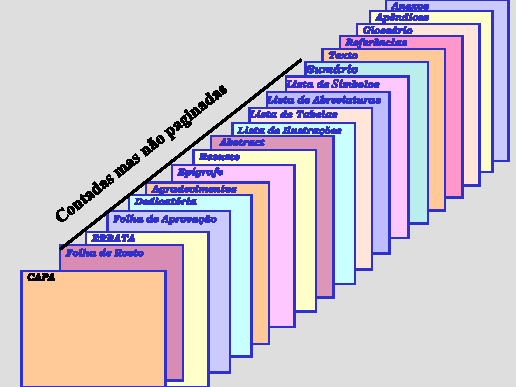
\includegraphics{images/imagem.pdf}
% 	\end{center}
% 	\fonte{Universidade Federal do Paraná (1996).}
% \end{figure}

% % ----------------------------------------------------------
% \subsection{Formatação do texto}
% % ----------------------------------------------------------

% No que diz respeito à estrutura do trabalho, recomenda-se que:
% \begin{alineas}
% 	\item o texto deve ser justificado, digitado em cor preta, podendo utilizar outras cores somente para as ilustrações;
% 	\item utilizar papel branco ou reciclado para impressão;
% 	\item os elementos pré-textuais devem iniciar no anverso da folha, com exceção da ficha catalográfica ou ficha de identificação da obra;
% 	\item os elementos textuais e pós-textuais devem ser digitados no anverso e verso das folhas, quando o trabalho for impresso. As seções primárias devem começar sempre em páginas ímpares, quando o trabalho for impresso. Deixar um espaço entre o título da seção/subseção e o texto e entre o texto e o título da subseção.
% \end{alineas}

% No \autoref{qua:Quadro_1} estão as especificações para a formatação do texto.

% \begin{quadro}[htb]
% 	\centering
% 	\caption{\label{qua:Quadro_1}Formatação do texto.}	
% 	\begin{tabular}{|l|p{11cm}|}
% 		\hline
% 		\textbf{Formato do papel} & A4.\\ \hline
% 		\textbf{Impressão}        & A norma recomenda que caso seja necessário imprimir, deve-se utilizar a frente e o verso da página.\\ \hline
% 		\textbf{Margens}          & Superior: 3, Inferior: 2, Interna: 3 e Externa: 2. Usar margens espelhadas quando o  trabalho for impresso.\\ \hline
% 		\textbf{Paginação}        & As páginas dos elementos pré-textuais devem ser contadas, mas não numeradas. Para trabalhos digitados somente no anverso, a numeração das páginas deve constar no canto superior direito da página, a 2 cm da borda, figurando a partir da primeira folha da  parte textual. Para trabalhos digitados no anverso e no verso, a numeração deve constar no canto superior direito, no anverso, e no canto superior esquerdo no verso.\\ \hline
% 		\textbf{Espaçamento}      & O texto deve ser redigido com espaçamento entre linhas 1,5, excetuando-se as citações de mais de três linhas, notas de rodapé, referências, legendas das ilustrações e das tabelas, natureza (tipo do trabalho, objetivo, nome da instituição a que é submetido e área de concentração), que devem ser digitados em espaço simples, com fonte menor. As referências devem ser separadas entre si por um espaço simples em branco.\\ \hline
% 		\textbf{Paginação}        & A contagem inicia na folha de rosto, mas se insere o número da página na introdução até o final do trabalho.\\ \hline
% 		\textbf{Fontes sugeridas} & Arial ou Times New Roman.\\ \hline
% 		\textbf{Tamanho da fonte} & \textbf{Fonte tamanho 12 para o texto}, incluindo os títulos das seções e subseções. As citações com mais de três linhas, notas de rodapé, paginação, dados internacionais de catalogação, legendas e fontes das ilustrações e das tabelas devem ser de tamanho menor. Adotamos, neste \textit{template} \textbf{fonte tamanho 10}.\\ \hline
% 		\textbf{Nota de rodapé}   & Devem ser digitadas dentro da margem, ficando separadas por um espaço simples por entre as linhas e por filete de 5 cm a partir da margem esquerda. A partir da segunda linha, devem ser alinhadas embaixo da primeira letra da primeira palavra da primeira linha.\\ \hline
% 	\end{tabular}
% 	\fonte{\textcite{NBR14724:2011}.}
% \end{quadro}

% % ----------------------------------------------------------
% \subsubsection{As ilustrações}
% % ----------------------------------------------------------

% Independentemente do tipo de ilustração (quadro, desenho, figura, fotografia, mapa, entre outros), a sua identificação aparece na parte superior, precedida da palavra designativa. 

% \begin{citacao}
% 	Após a ilustração, na parte inferior, indicar a fonte consultada (elemento obrigatório, mesmo que seja produção do próprio autor), legenda, notas e outras informações necessárias à sua compreensão (se houver). A ilustração deve ser citada no texto e inserida o mais próximo possível do texto a que se refere. \cite[p. 11]{NBR14724:2011}.
% \end{citacao}

% % ----------------------------------------------------------
% \subsubsection{Equações e fórmulas}
% % ----------------------------------------------------------

% As equações e fórmulas devem ser destacadas no texto para facilitar a leitura.  Para numerá-las, usar algarismos arábicos entre parênteses e alinhados à direita. Pode-se adotar uma entrelinha maior do que a usada no texto \cite{NBR14724:2011}.

% Exemplos, \autoref{eq:Eq_1} e \autoref{eq:Eq_2}. Observe que o comando \verb|\gls{}| é usado para utilizar para criar um \emph{hyperlink} com a definição do símbolo na lista de símbolos (veja linha 153 de \emph{main.tex}.

% \begin{equation}
% \label{eq:Eq_1}
% \gls{C} = 2 \gls{pi} \gls{r} \sqrt{\gamma} + 10 \, \text{.}
% \end{equation}

% \begin{equation}
% \label{eq:Eq_2}
% \gls{A} = \gls{pi} \gls{r}^2 \, \text{.}
% \end{equation}

% \noindent Aqui não há recuo porque o parágrafo não terminou, apenas foi iniciada uma nova frase após a equação. As equações fazem parte do texto, portanto estão sujeitas à pontuação (ponto final, vírgula etc.).

% % ----------------------------------------------------------
% \subsubsubsection{Exemplo tabela}
% % ----------------------------------------------------------

% De acordo com \textcite{ibge1993}, tabela é uma forma não discursiva de apresentar informações em que os números representam a informação central. Ver \autoref{tab:Tab_1}.

% \begin{table}[htb]
% 	\ABNTEXfontereduzida
% 	\caption{\label{tab:Tab_1}Médias concentrações urbanas 2010-2011.}
% 	\begin{tabular}{@{}p{3.0cm}p{1.5cm}p{2cm}p{2.5cm}p{2.5cm}p{2.5cm}@{}}
% 		\toprule
% 		\textbf{Média concentração urbana} & \multicolumn{2}{l}{\textbf{População}} & \textbf{Produto Interno Bruto – PIB (bilhões R\$)} & \textbf{Número de empresas} & \textbf{Número de unidades locais} \\ \midrule
% 		\textbf{Nome}                      & \textbf{Total}   & \textbf{No Brasil}  &                                                   &                             & \\
% 		Ji-Paraná (RO)                     & 116 610          & 116 610             & 1,686                                             & 2 734                       & 3 082 \\
% 		Parintins (AM)                     & 102 033          & 102 033             & 0,675                                             & 634                         & 683 \\
% 		Boa Vista (RR)                     & 298 215          & 298 215             & 4,823                                             & 4 852                       & 5 187 \\
% 		Bragança (PA)                      & 113 227          & 113 227             & 0,452                                             & 654                         & 686 \\ \bottomrule
% 	\end{tabular}
% 	\fonte{\textcite{ibge2016}.}
% \end{table}